\tocless\subsection{Hoare Logic}

As a starting point in proving correctness, or generally properties of computer programs, Hoare \cite{hoare} explains how to use deductive reasoning in applying inference rules to a set of predefined language axioms. He specifies the use of what was later on referred to as a ``Hoare triple" of the shape $\triple{P}{C}{Q}$ where $P$ and $Q$ are first-order assertions while $C$ is the program executed. $P$ is called the precondition of $C$ while $Q$ is its postcondition. The triple thus describes that whenever the assertion $P$ holds before $C$ runs and at some point terminates, then $Q$ will hold on its completion. The kind of logic adopted, allows to reason about relatively simple programs involving integers and local variables living in the \textit{stack} of a function. Classic proofs performed using Hoare logic take the form of a proof tree with axioms as leaves and rules as intermediate steps. Such notation has the downside that complete proofs tend to explode in size. For this reason, proof sketches are utilized. They represent the holding assertions before and after every command that appears in the analyzed code. We can see an example of such in Figure \ref{fig:abshoare}.
\begin{center}
	\begin{gather*}
		\begin{array}{l}
		\specline{\top} \\
		\pfunctions{abs}{\pvar{x}} \\
			\quad \passign{\pvar{r}}{\pvar{x}}; \\
			\quad \specline{\pvar{x} = \pvar{r}} \\
			\quad \pifelses{\pvar{x} < 0} \\
				\quad \quad \specline{\pvar{x} < 0 \land \pvar{x} = \pvar{r}} \\
				\quad \quad \passign{\pvar{r}}{-\pvar{x}}; \\
				\quad \quad \specline{\pvar{x} < 0 \land \pvar{r} = - \pvar{x}} \\
				\quad \quad \specline{(\pvar{x} < 0 \land \pvar{r} = -\pvar{x}) \lor (\pvar{x} \geq 0 \land \pvar{r} = \pvar{x})} \\
			\quad \pifelsem \\
				\quad \quad \specline{\pvar{x} \geq 0 \land \pvar{x} = \pvar{r}} \\
				\quad \quad \pskip; \\
				\quad \quad \specline{\pvar{x} \geq 0 \land \pvar{x} = \pvar{r}} \\
				\quad \quad \specline{(\pvar{x} < 0 \land \pvar{r} = -\pvar{x}) \lor (\pvar{x} \geq 0 \land \pvar{r} = \pvar{x})} \\
			\quad \pifelsee \\
			\quad \specline{(\pvar{x} < 0 \land \pvar{r} = -\pvar{x}) \lor (\pvar{x} \geq 0 \land \pvar{r} = \pvar{x})} \\
			\quad \preturn{\pvar{r}}; \\
		\pfunctione \\
		\specline{(\pvar{x} < 0 \land \pvar{ret} = -\pvar{x}) \lor (\pvar{x} \geq 0 \land \pvar{ret} = \pvar{x})} \\
		\end{array}
	\end{gather*}
	\captionof{figure}{A proof sketch of the absolute value function using Hoare logic.}
	\label{fig:abshoare} 
\end{center}

The $\mathtt{abs}(\pvar{x})$ function simply returns the absolute value of the input argument $\pvar{x}$. We notice that the procedure's precondition is $\top$ ($true$), which means that there is no particular assertion which needs to hold in order for the code to perform its task. On the other hand, the postcondition states that the return value, which is referred to using a special variable named $\pvar{ret}$, will effectively be the absolute value of $\pvar{x}$. Note how the postcondition of every command in a sequence becomes the precondition of the following one, respecting the rule specified in \cite{hoare}.

\tocless\subsection{Owicki-Gries}

In a concurrent setting, the first approach that allowed reasoning of programs was presented in \cite{owicki} and is referred to as the ``Owicki-Gries" method from the name of its authors. Its main contribution is the parallel composition rule.

\[
	\infer[\textsc{Owicki-Gries}]
	{
		\vdash \triple{P_1 \land P_2}{C_1\ ||\ C_2}{Q_1 \land Q_2}
	}
	{
		\vdash \triple{P_1}{C_1}{Q_1} &
		\vdash \triple{P_2}{C_2}{Q_2} &
		\textsf{interference-free}
	}
\]

The rule states that we perform a regular sequential proof for each of the threads that are composed together and the resulting postcondition will be the conjunction of all the components' ones. This holds as long as the proofs of the individual thread runs are not interfering with each other. In other words, every intermediate assertion between atomic commands in the sequential proof of $C_1$ must be kept valid by the actions of $C_2$ and vice versa \cite{viktor}.
\begin{center}
\[\footnotesize
\begin{array}{c}
\infer[\textsc{Cons}]
{
	\triple
	{\pvar{x} = 0}
	{\passign{\pvar{x}}{\pvar{x} + 1}\ ||\ \passign{\pvar{x}}{\pvar{x} + 2}}
	{\pvar{x} = 3}
}
{
	\infer[\textsc{Owicki-Gries}]
	{
		\triple
		{\pvar{x} = 0 \land \pvar{x} = 0}
		{\passign{\pvar{x}}{\pvar{x} + 1}\ ||\ \passign{\pvar{x}}{\pvar{x} + 2}}
		{(\pvar{x} = 1 \lor \pvar{x} = 3) \land (\pvar{x} = 2 \lor \pvar{x} = 3)}
	}
	{
		(\dag)
		\ \ \ \ \ \ \ \ \ \ \ \ \ \ \ \	
		(\spadesuit)
	}
}
\\[1.5em]
(\dag) =
\infer[\textsc{Cons}]
		{
			\triple
			{\pvar{x} = 0}
			{\passign{\pvar{x}}{\pvar{x} + 1}}
			{\pvar{x} = 1 \lor \pvar{x} = 3}
		}
		{
			\infer[\textsc{Assign}]
			{
				\triple
				{\pvar{x} = 0 \lor \pvar{x} = 2}
				{\passign{\pvar{x}}{\pvar{x} + 1}}
				{\pvar{x} = 1 \lor \pvar{x} = 3}
			}
			{\ldots}		
		}
\\[1.5em]
(\spadesuit) = 
\infer[\textsc{Cons}]
		{
			\triple
			{\pvar{x} = 0}
			{\passign{\pvar{x}}{\pvar{x} + 2}}
			{\pvar{x} = 2 \lor \pvar{x} = 3}
		}
		{
			\infer[\textsc{Assign}]
			{
				\triple
				{\pvar{x} = 0 \lor \pvar{x} = 1}
				{\passign{\pvar{x}}{\pvar{x} + 2}}
				{\pvar{x} = 2 \lor \pvar{x} = 3}
			}
			{\ldots}		
		}
\\[1.5em]
\infer[\textsc{Cons}]
	{
		\triple
		{P}
		{C}
		{Q}
	}
	{
		P \Rightarrow P' &
		\triple
		{P'}
		{C}
		{Q'} &
		Q' \Rightarrow Q
	}
\end{array}
\]
\captionof{figure}{Partial proof tree of a parallel program incrementing variable $\pvar{x}$ which also uses the \textsc{Cons} rule (provided).}
\end{center}

The method's main burden is the \textsf{interference-free} constraint which makes non-trivial commands very complicated to prove. As a consequence, most specifications that satisfy the requirement will be too weak to prove any interesting properties about the concurrent code. This is the reason why such a method is only able to give stronger specifications using auxiliary or ghost variables whose task is to keep track of past program states. In addition, the actual code needs to be augmented with statements that refer to the ghost variables themselves. Any modular use of proofs that involve auxiliary variables would require new specifications, since the number of variables needed to express strong specifications would increase based on the way the module is used (e.g. the number of threads running). This becomes clear by looking at an example of two threads incrementing the same counter concurrently. We first define the counter's methods and then show a summarized proof of clients' usage through ghost variables \cite{modularsteps}.
\begin{gather*}
\begin{array}{@{}l@{\qquad}l@{\qquad}l@{}}
\begin{array}{@{}l@{}}
\pfunctions{makeCounter}{} \\
\quad \palloc{\pvar{c}}{1}; \\
\quad \pmutate{\pvar{c}}{0}; \\
\quad \preturn{\pvar{c}}; \\
\pfunctione
\end{array}
&
\begin{array}{@{}l@{}}
\pfunctions{increment}{\pvar{c}} \\
\quad \texttt{do } \{ \\
	\quad \quad \pderef{\pvar{n}}{\pvar{c}}; \\
	\quad \quad \pfuncall{\pvar{b}}{CAS}{\pvar{c}, \pvar{n}, \pvar{n} + 1}; \\
\quad \} \texttt{ while }(\pvar{b} = 0); \\
\quad \preturn{\pvar{n}}; \\
\pfunctione
\end{array}
\end{array} \\ \\
\pfuncall{\pvar{c}}{makeCounter}{};
\color{ForestGreen}\passign{\pvar{inc}_1}{0};
\passign{\pvar{inc}_2}{0}; \\
\color{blue} \{ \cell{\pvar{c}}{0} \land \pvar{inc}_1 = 0 \land \pvar{inc}_2 = 0 \} \\
\begin{array}{c || c}
\begin{array}{l}
\color{blue} \{ \cell{\pvar{c}}{\pvar{inc}_1 + \pvar{inc}_2} \land \pvar{inc}_1 = 0 \} \\
\texttt{do } \{ \\
	\quad \pderef{\pvar{n}}{\pvar{c}}; \\
	\quad \patomic{\pfuncall{\pvar{b}}{CAS}{\pvar{c}, \pvar{n}, \pvar{n} + 1}; \\
		\quad \quad \textcolor{ForestGreen}{\pifelses{\pvar{b}} \pvar{inc}_1\texttt{++}\pifelsee}} \\
\} \texttt{ while }(\pvar{b} = 0); \\
\color{blue} \{ \cell{\pvar{c}}{\pvar{inc}_1 + \pvar{inc}_2} \land \pvar{inc}_1 = 1 \} \\
\end{array}
&
\begin{array}{l}
\color{blue} \{ \cell{\pvar{c}}{\pvar{inc}_1 + \pvar{inc}_2} \land \pvar{inc}_2 = 0 \} \\
\texttt{do } \{ \\
	\quad \pderef{\pvar{n}'}{\pvar{c}}; \\
	\quad \patomic{\pfuncall{\pvar{b}'}{CAS}{\pvar{c}, \pvar{n}', \pvar{n}' + 1}; \\
		\quad \quad \textcolor{ForestGreen}{\pifelses{\pvar{b}'} \pvar{inc}_2\texttt{++}\pifelsee}} \\
\} \texttt{ while }(\pvar{b}' = 0); \\
\color{blue} \{ \cell{\pvar{c}}{\pvar{inc}_1 + \pvar{inc}_2} \land \pvar{inc}_2 = 1 \} \\
\end{array}
\end{array} \\
\color{blue} \{ \cell{\pvar{c}}{\pvar{inc}_1 + \pvar{inc}_2} \land \pvar{inc}_1 = 1 \land \pvar{inc}_2 = 1 \} \\
\color{blue} \{ \cell{\pvar{c}}{2} \}
\end{gather*}

As we can see, the parts of code in \textcolor{ForestGreen}{green} are auxiliary, i.e. they are not part of the executed code but are there to aid the proof. We use them to build the invariant that each of the two concurrent commands will use to prove its postcondition. In fact, at any point in the concurrent execution, the counter value will be the sum of the two auxiliary variables. Note that the increments to the ghost variables $\mathtt{inc}_1$ and $\mathtt{inc}_2$ must happen atomically with the respective $\mathtt{CAS}$ commands and this is the reason why they are included in an atomic context $\patomic{-}$.

If we now were to prove three separate threads incrementing the same counter in parallel, we would have to redo the proof, adding a new auxiliary variable $\mathtt{inc}_3$ and changing the invariants in all of the other bodies. The solution proposed is therefore not compositional. This implies that whenever we add a new method to a verified module which interacts with some shared state, we need to cross check every new command with all the others already present.

\tocless\subsection{Rely/Guarantee}

Jones \cite{jones} introduces a way of explicitly stating the interference coming from the environment as part of concurrent composition of code. This replaces the implicit and tedious side condition in the parallel rule of the ``Owicki-Gries" method. The result is rely/guarantee reasoning which is a compositional method. The specifications that arise from the use of such technique, adopt binary relations to express how the state might change as a result of the running thread's or the environment's actions.

\begin{center}
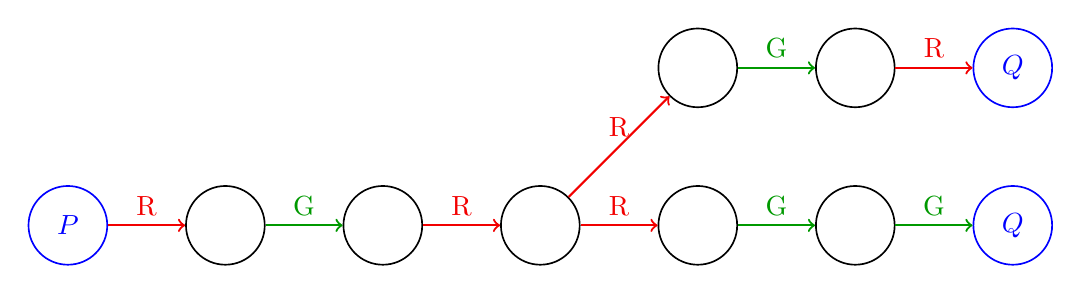
\begin{tikzpicture}[->, semithick]
\tikzset{
    prepost/.style= {circle, draw=blue, color=blue, minimum size=1.0cm},
    pstate/.style= {circle, draw=black, minimum size=1.0cm},
    prel/.style= {above, black!5!red, thick},
    pguar/.style= {above, black!40!green, thick},
}

\node[prepost] (P) at (0,0) {$P$};
\node[pstate] (s1) at (2,0) {};
\node[pstate] (s2) at (4,0) {};
\node[pstate] (s3) at (6,0) {};
\node[pstate] (s4) at (8,0) {};
\node[pstate] (s5) at (10,0) {};
\node[prepost] (s6) at (12,0) {$Q$};

\node[pstate] (s8) at (8,2) {};
\node[pstate] (s9) at (10,2) {};
\node[prepost] (s10) at (12,2) {$Q$};

\draw
(P) edge[prel] node {R} (s1)
(s1) edge[pguar] node {G} (s2)
(s2) edge[prel] node {R} (s3)
(s3) edge[prel] node {R} (s4)
(s4) edge[pguar] node {G} (s5)
(s5) edge[pguar] node {G} (s6)
(s3) edge[prel] node {R} (s8)
(s8) edge[pguar] node {G} (s9)
(s9) edge[prel] node {R} (s10);
\end{tikzpicture}
\captionof{figure}{An interleaving of environment and thread actions abstracted using rely/guarantee relations.}
\end{center}

A predicate $P$ that refers to the structure of a single state, describes a set of possible states, while binary relations represent a set of transitions that can happen in the system \cite{viktor}. The latter are predicates of the form $P_a(\vec{\sigma}, \sigma)$ that relate the state before action $a$ to the one right after. Given a single predicate we can define the two-state relation by placing no constraint on the old state, $P(\sigma) \triangleq P(\vec{\sigma}, \sigma)$ or on the other hand by not restricting the new state $\sigma$, $P(\vec{\sigma}) \triangleq P(\vec{\sigma}, \sigma)$. State relations can be sequentially composed in order to reflect the effect of actual program commands as follows $(P; Q)(\vec{\sigma}, \sigma) \triangleq \exists \alpha \ldotp P(\vec{\sigma}, \alpha) \land Q(\alpha, \sigma)$. We can now define that a binary relation $P$ is stable under another relation $Q$ if and only if $(P; Q) \Rightarrow P \land (Q; P) \Rightarrow P$ which means that whenever an action in $Q$ is done before or after a transition in $P$, this must not invalidate $P$ itself.

Every specification will now take the form $\triplena{R, G}{P}{C}{Q}$ and include the standard pre and postconditions, plus $R$ and $G$, the rely and guarantee relations. The rely relation models all actions that the environment can perform while the guarantee one describes what the thread executing $C$ has the ability to do. In order for the proof to be valid, $G$ needs to be stable under the interference of $R$. Stability is only explicitly checked at the atomic command level \cite{viktor} as the following inference rule describes.

\[
\infer[\textsc{RG-Atomic}]
{
	\triplena{R, G}{P}{\patomic{C}}{Q}
}
{
	\triplena{\mathsf{ID}, \top}{P}{C}{Q}
	\ \
	(P, Q) \in G
	\ \
	\pred{stable}{P, R}
	\ \
	\pred{stable}{Q, R}
}
\]

Given that $C$ executes atomically, there can be no interference from the environment, so $R \equiv \mathsf{ID}$, the identity relation, meaning that the state will be kept as it is. On the other hand, the guarantee relation $G \equiv \top$, allows any operation, although, as part of the premiss, we require the state pair $(P, Q)$ to be part of the original guarantee relation. The hard requirement is the explicit check of stability of $P$ and $Q$ under relation $R$.

\[
\infer[\textsc{RG-Par}]
{
	\triplena{R, G_1 \cup G_2}{P_1 \land P_2}{C_1\ ||\ C_2}{Q_1 \land Q_2}
}
{
	\triplena{R \cup G_2, G_1}{P_1}{C_1}{Q_1}
	\ \
	\triplena{R \cup G_1, G_2}{P_2}{C_2}{Q_2}
}
\]

Commands are composed in parallel using the \textsc{RG-Par} rule that makes the guarantee of the first command be part of the rely relation of the second one and vice-versa. This makes sure that we model all interference coming from concurrent threads.